% -*- latex -*-
%-----------------------------------------------------------------------
%;  Copyright (C) 2000-2001
%;  Associated Universities, Inc. Washington DC, USA.
%;
%;  This program is free software; you can redistribute it and/or
%;  modify it under the terms of the GNU General Public License as
%;  published by the Free Software Foundation; either version 2 of
%;  the License, or (at your option) any later version.
%;
%;  This program is distributed in the hope that it will be useful,
%;  but WITHOUT ANY WARRANTY; without even the implied warranty of
%;  MERCHANTABILITY or FITNESS FOR A PARTICULAR PURPOSE.  See the
%;  GNU General Public License for more details.
%;
%;  You should have received a copy of the GNU General Public
%;  License along with this program; if not, write to the Free
%;  Software Foundation, Inc., 675 Massachusetts Ave, Cambridge,
%;  MA 02139, USA.
%;
%;  Correspondence concerning AIPS should be addressed as follows:
%;          Internet email: aipsmail@nrao.edu.
%;          Postal address: AIPS Project Office
%;                          National Radio Astronomy Observatory
%;                          520 Edgemont Road
%;                          Charlottesville, VA 22903-2475 USA
%-----------------------------------------------------------------------
%Body of AIPSletter for 31 December 2000

\documentclass[twoside]{article}
\usepackage{graphics}

\newcommand{\AIPRELEASE}{December 31, 2000}
\newcommand{\AIPVOLUME}{Volume XX}
\newcommand{\AIPNUMBER}{Number 2}
\newcommand{\RELEASENAME}{{\tt 31DEC00}}
\newcommand{\OLDNAME}{{\tt 15OCT99}}
\newcommand{\NEXTNAME}{{\tt 31DEC01}}

%macros and title page format for the \AIPS\ letter.
\input LET98.MAC
%\input psfig

\newcommand{\MYSpace}{-11pt}

\normalstyle

\section{General developments in \AIPS}

\subsection{Current and future releases}

We had not expected to have any further formal releases of \AIPS\@.
Instead, \AIPS\ has been available as the {\tt 31DEC99} version since
October 1999.  However, \AIPS\ continues to be heavily used and will
likely remain in use with limited development for some years to come.
Therefore, we have reinstated the old practice of having formal \AIPS\
releases.  These will be done on an annual basis and there will be a
binary release only for Solaris and Linux.  All architectures can do a
full installation from the source files.  Therefore, we have changed
{\tt 31DEC99} to {\tt 31DEC00} and it is now, or soon will be,
available as a frozen release.  Tape and CDrom copies will be
available; see the \AIPS\ web page or use the order form at the back
of this \Aipsletter.

The next release will be called {\tt 15DEC01} and remains under
development by the (reduced) \AIPS\ Group.  You may fetch and install
a complete copy of this version at any time.  Having done so, you may
update your installation whenever you want either as a whole or by
running the so-called ``midnight job'' which uses transaction files to
copy and compile the code selectively based on the code changes and
compilations we have done.  We expect users to take the source-only
version of {\tt 15DEC01} \AIPS\ over the Internet (via
\emph{anonymous} ftp).

\AIPS\ is now copyright \copyright\ 1995 through 2000 by Associated
Universities, Inc., NRAO's parent corporation, but may be made freely
available under the terms of the Free Software Foundation's General
Public License (GPL)\@.  This means that User Agreements are no longer
required, that \AIPS\ may be obtained via anonymous ftp without
contacting NRAO, and that the software may be redistributed (and/or
modified), under certain conditions.  The full text of the GPL can be
found in the \texttt{15JUL95} \Aipsletter.

\subsection{Personnel}

The \AIPS\ Group, none of whom work full time on \AIPS, consisted a
year ago of Chris Flatters, Ketan Desai, and Leonia Kogan doing
programming and user support at the AOC in Socorro and Eric Greisen
and Pat Murphy performing similar roles in Charlottesville.  Ernie
Allen handles data base and shipping chores for the Group.  This was a
pretty minimal group to support such a large and widespread software
package.  Unfortunately, this group has been eroding.  Pat is also
Head of the Charlottesville Computing Division, a nearly full-time job.
This summer, Chris left the group to join Ketan (who left in the
spring) both to find greener pastures working in the New York City
area.  We wish them well in their new endeavors, but their departures
have left us well below minimum strength.  The position advertised,
among other places, in the previous \Aipsletter\ received very few
applicants and was not filled.

     Three actions are being taken to address these problems.  First,
Eric has moved to Socorro on a permanent basis.  Second, with the bulk
of the applications support now being done in Socorro, Jim Ulvestad
replaced Tony Beasley as the nominal supervisor of the \AIPS\ Group in
May.  Third, despite NRAO's current financial problems, a position to
replace Ketan and/or Chris was announced and advertised via {\tt
bananas}, various web pages, and the AAS\@.  Amy Mioduszewski has
accepted the position and will begin work in Socorro in mid January.

\section{Improvements of interest to users in \RELEASENAME}

We expect to continue publishing the  \Aipsletter\ approximately every
six months along with the annual releases.  Despite the reduction and
disruption in personnel, there have been a surprising number of
changes in {\tt 31DEC00} over the past six months.  There are three
new tasks: {\tt FACES} to convert a coordinate and NVSS catalog into
an initial set of images and Clean components, {\tt OOSRT} to sort
\uv\ data, {\tt MATCH} to change a \uv\ data set to have {\tt FREQID},
source, and antenna numbers matching another data set, and {\tt PBEAM}
to fit observations of the primary beam.  New verbs are {\tt COPIXEL}
to convert between physical and pixel coordinates and {\tt\ $\sim$\ },
the tilde sign, to assign a list of values to an array starting at any
specified subscript.

{\tt 31DEC00} treats data weights in different ways than earlier
releases (see below) and has a variety of changed adverb names and the
like.  Other than these relatively minor ways, {\tt 31DEC00} is
compatible in all major ways with the other 1999 and {\tt 15OCT98}
releases.  There are significant incompatibilities with older
versions.

\subsection{Imaging and Clean models}

\subsubsection{IMAGR}

{\tt IMAGR} was given the option to remake all fields automatically
every $n$ major cycles in the ``{\tt OVERLAP }$n$'' mode, where $n >
2$ is the (new) user-specified value of {\tt OVERLAP}\@.  This option
is likely to be used when Cleaning without use of the TV\@.  The task
was changed to restore only the width-zero fields when Cleaning with
the multi-resolution algorithm.  The method of restoration used means
that the other versions of the fields only differ by having smoother
noise.  Whenever {\tt IMAGR} has just computed all fields in the {\tt
OVERLAP} $\ge 2$ mode, it will load the TV with the field it will
Clean next (unless the user changes the boxes).  Previously, it loaded
the last one displayed.  {\tt IMAGR} was also given the ability to
have {\it no} Clean boxes in a field, indicated initially by setting
{\tt FLDSIZ} for that field less than zero.  The final Cleaned flux in
each field is now reported..

A few bugs affecting only {\tt IMAGR} were fixed.  Tapering was not
done when natural weighting was specified.  When ``3D'' imaging
using {\tt OVERLAP} $< 2$, the computation of the histogram of
residuals was done only on the first field.  This was able to confuse
things badly, allowing way more than {\tt MAXPIXEL} pixels to be
loaded to the AP and ending up in nearly infinite loops.  Now the
histogram is done over all images.  {\tt IMAGR} was filtering the
Clean Components if that option was requested at the beginning, even
if a {\tt TELL} was used to turn it off later.  A bug was corrected in
the gridding of data.  This bug was most likely to affect sparse data
being gridded for a large image using a small pseudo-AP memory.

\subsubsection{Clean-component modeling}

Many of the same routines are used to subtract Clean components while
finding them in {\tt IMAGR} and later to use them for modeling and
calibration in {\tt UVSUB}, {\tt CALIB}, and numerous other tasks.
Some potentially significant bugs were found and corrected.  A change
to allow parallel operation in DFT point component division changed
the meaning of the array used to scale from the first to later
frequencies.  Unfortunately, the calling routines that prepare this
array and other similar {\tt Q} routines that also use it were not
changed.  They are now all consistent.  This bug could, among other
things, reduce the ability of a Clean model to eliminate a distant
interfering source.

The gridded subtraction routine for time-baseline sorted data had an
annoying habit in large cases of looping through all the data once for
each spectral channel and IF and each of several swaths in the \uv\
plane.  The routine, {\tt ALGSTB}, was changed to overlap the swaths
to allow all frequencies to be subtracted at once.

For some time, the model subtraction and division using a
user-specified {\tt SMODEL} has failed.  This option is only supported
by the DFT routines, but the gridded ones were called.  Therefore, the
output data did not have the model subtracted or divided.

The model-using tasks were changed to allow use of the model from one
or more consecutive fields beginning with field $n$, where $n$ does
not have to be 1.  Previously, the new naming convention for fields did
not allow for excluding low-numbered fields from the model.

\subsubsection{Using survey catalogs}

The task {\tt SETFC} is designed to determine the ``faces'' or fields
needed to image the primary beam area fully and to image any
interfering sources if they are likely to be strong enough.  It writes
a {\tt BOXFILE} for use by {\tt IMAGR}\@.  {\tt SETFC} has been
improved since the last \Aipsletter\ by adding 1950 as well as 2000
catalogs, by adding a flux cutoff control, and by including the
Westerbork Sky Survey (WENSS) as a catalog as well as several NRAO VLA
D-Array Survey (NVSS) flux-limited catalogs.  Also inserted were
schemes suggested by Bill Cotton for selecting cell and image sizes
and for positioning the ``fly's eye'' faces to cover the primary beam.
The task now writes to the {\tt BOXFILE} an inscribed circular Clean
box for each of the fly's eye faces and. optionally, small circular
Clean boxes for each of the interfering sources.  A new task called
{\tt FACES} has been written.  It is designed to read the catalog
files and create a set of images with associated Clean components
files based on what it finds in the catalog.  These {\tt CC} files may
then be used as an initial guess to calibrate the first self-cal cycle
of the corresponding observation.  It uses Bill's schemes as well.

Both of these tasks plus {\tt PBCOR} and {\tt PATGN} need to have a
correct antenna power pattern.  The beam computation has been pulled
into a single subroutine (called {\tt PBCALC}) used by all these
tasks.  To improve the form used and the default values, new
observations have been made with the VLA by Rick Perley and a new
task ({\tt PBEAM}) has been written by Leonia Kogan to fit the
observations.  The results of the fitting have been installed in
these tasks and the fitting task has been made available.  Wavelengths
longer than 21cm remain to be done with the new tools.

\subsubsection{UVCON}

{\tt UVCON} generates a \uv\ data set from a user-specified array
geometry and a source model specified in the usual ways (Clean
components, image, or {\tt SMODEL})\@.  DFT is used to compute the
model visibilities.  This task has been used to study ALMA
configurations and other array design questions.  In June, the ability
to study the effects of pointing error was added.  Three types of
primary beam are offered: flat illumination (like the VLA),
illumination down by 10db at the dish edge, and illumination down by
15db.  Three kinds of pointing error are offered as well: a constant
error for all antennas and times (\ie\ a source position error), an
error that is constant in time but random among antennas, and errors
that are random in time and between antennas.  Preliminary results
from this task suggest that modest random pointing errors are less
important than were previously thought.

\subsubsection{Other imaging changes}

\begin{description}
\myitem{HGEOM} and {\tt OHGEO} gave the user little control over the
           reference pixel in the output image.  The output reference
           pixel is now controlled by adverbs and the defaults were
           changed to be more consistent.  The output header in {\tt
           OHGEO} was corrected to contain the coordinates of the
           first image for axes 3--7.  An I.O error, which caused the
           output of all {\tt *GEOM} tasks to be wrong for large
           cubes, was corrected.
\myitem{XTRAN} was changed to give it a {\tt DOOUT = -2} mode to test
           what it would do when just changing the header.  The
           computation of header parameters was corrected and a second
           report of their accuracy compared to the full fit was
           added.  The re-gridding was changed to use the full $x$ and
           $y$ fits even when only three parameters are found.  This
           seems to handle skew to some extent.  Corrected handling of
           {\tt BLC} and {\tt TRC} and made the task use only those
           star positions inside the sub-image being fit rather than
           all the positions in the text file.
\myitem{CONVL} needed larger buffers to handle images up to 8192 on a
           side.  It cannot handle larger images and a warning about
           this was added.
\myitem{IRING} had its coordinates fixed just before the last
           \Aipsletter, but that left the beam area negative.
           Corrected this and fixed an error handling {\tt BLC}\@.
\myitem{FLATN} has been upgraded to do both multiple pointings, using
           the new beam pattern routine, and multiple fields.  {\tt
           LTESS} plus {\tt HGEOM} may no longer be required for
           mosaics.
\end{description}

\subsection{Interferometric data handling}

\subsubsection{VLA data weights}

Data weights are supposed to be, or at least be proportional to, one
over the rms uncertainty squared.  In the past, there seemed to be
little, if any, effective way to measure this, so a simple count of
the number of 10-second records was used with VLA data.  The on-line
measurements of system temperature are known to suffer from systematic
errors in their calibration and so were thought not to be useful.
However, Ketan Desai (\AIPS\ Memo 103) pointed out that the ``nominal
sensitivity'' which is measured on-line is the scaling applied to the
visibilities to convert them roughly to deciJy.  The nominal
sensitivity is then a measure of the rms uncertainty that suffers
from the {\it same} calibration errors as the data themselves.  Thus,
if the calibrations found by {\tt CALIB} and friends are applied to
weights initially set by the nominal sensitivity then, after
calibration, these weights will be proportional to $1/\sigma^2$ as
desired.  In the previous \Aipsletter, we described how the VLA task
{\tt FILLM} is able to set these weights and how all calibration
application tasks can use {\tt DOCALIB=2} to signal the desire to
calibrate both data and weights.  The {\tt DOWEIGHT} adverb has since
been added to {\tt FILLM} after this scheme was found to be
effective.  Compression of \uv\ data eliminates the differences in
weights between IFs and polarizations within each data sample.  Since,
in the new schjeme, these weights can differ substantially,
uncompressed data should probably be used where feasible.

On July 7, 2000, Chris Carilli reported:

{\it As promised, the following is a summary of the use of the ``VLA
weight cal transfer' for some recent 43 GHz data from the VLA.
Overall, the process works properly, and will make the calibration,
flagging, and imaging procedures significantly easier, and improve the
sensitivity of the final image.

In review, the process is needed in order to have proper data weights
based on measured $T_{sys}$ values and antenna gains.  The current
implementation is very simple, requiring a value of {\tt CPARM(2) = 8}
(or {\tt DOWEIGHT = 1}) in {\tt FILLM}, then follow the normal
calibration procedure, then use {\tt DOCAL = 2} in {\tt SPLIT}\@.
This process is extremely useful at 43 GHz and 22 GHz, where the
system response varies by more than a factor two from the best to the
worst antennas, but is also useful at 1.4 GHz where the $T_{sys}$
increases due to spill-over at low elevation.

I loaded data from project AI79 (high redshift CO at 43 GHz) in both
the usual way, and in the new proper cal-transfer way.  I ran {\tt
CALIB} and found that antennas 17, 20, and 24 all had much higher
(poorer) gains than most antennas, by a factor between 3 and 5. After
splitting with {\tt DOCAL = 2}, the weights for baselines involving
these antennas were lower by similar factors than for other baselines.
A good example of this was antenna 26, which had a gain factor about
two times higher than good antennas. After splitting, baselines
involving antenna 26 had weights about two times lower than those for
good antennas.

In terms of image noise, the results for the rms on NA weighted images
are:
\begin{center}
\begin{tabular}{lr}
All data with weight transfer:                & $0.178$ mJy/beam\\
All data without weight transfer:             & $0.310$ mJy/beam\\
Without ant 17,20,24 with weight transfer:    & $0.185$ mJy/beam\\
Without ant 17,20,24 without weight transfer: & $0.220$ mJy/beam
\end{tabular}
\end{center}}

\subsubsection{Calibration problems}

\begin{description}
\myitem{CALIB} takes the times from the {\tt NX} table and rounds them
         outward by a little to be certain to include all the data
         from that scan.  Unfortunately, a ``little'' was 4.32 sec,
         rather more than the comment claimed, and able to overlap
         into the next scan in phase-switching experiments (which may
         be separated by only 3 seconds).  The result was a series of
         good solutions separated by rather poor ones from the couple
         of seconds of overlap.
\myitem{CL table} and {\tt BP} table weights were not examined by most
         calibration application routines although they are used to
         flag solutions by {\tt SNEDT} and other routines.
\myitem{NX tables} may be missing and the calibration routines try to
         function without them.  This is actually the normal case for
         single-source files, but now gets a warning on multi-source
         files.  Source-specific data selection and flagging were
         failing in this case and required generalization.
\myitem{INDXR} was capable of getting the wrong antenna and subarray
         numbers from the internal code in, one hopes, rare
         circumstances.
\myitem{CALIB} now supports the minus sign convention for {\tt DOFIT}
         to mean all but those listed.
\myitem{GETJY} had an error causing the antenna deselection option to
         fail on some computers.
\myitem{FG table} copying with {\tt UVCOP} and other tasks failed to
         delete records correctly when they fell outside the selected
         range of IF and spectral channel.
\end{description}

\subsubsection{Simplified VLBI data reduction}

A new {\tt RUN} file called {\tt VLBAUTIL} has been added to the
system along with all supporting {\tt HELP} files including one for
{\tt VLBAUTIL} itself.  The procedures contained in the file are
intended to simplify the reduction of normal VLBA data.  The
procedures are
\begin{center}
\begin{tabular}{ll}
{\tt VLBALOAD} & loads VLBA data with simplified inputs \\
{\tt VLBASUBS} & finds subarrays in VLBA data \\
{\tt VLBAMCAL} & removes redundant calibration data from tables \\
{\tt VLBAFQS } & copies frequency IDs to separate files \\
{\tt VLBAFPOL} & fixes polarization labelling for common cases \\
{\tt VLBACALA} & determines a-priori amplitude corrections \\
{\tt VLBAPANG} & determines phase corrections for parallactic angles \\
\end{tabular}
\end{center}

A new appendix to the \Cookbook\ has been written to represent a
simplified approach to VLBA data reduction.  It has been released as a
VLBA Memo (see below) and will become part of the \Cookbook\ shortly.
This memo includes a brief description of when the above procedures
should be run in data reduction process.  Within the next few months
we plan to add a procedure to apply pulse-cal tones and to improve the
procedure used for polarization D-term (leakage) calibration.

\subsubsection{VLBI data handling}

\begin{description}
\myitem{MATCH} is a new task.  It copies a data set renumbering the
          sources, antennas, and {\tt FREQID}s to match those in a
          second data set.  The task may be needed to align data sets
          from multiple files or extra-wide bandwidth observations
          processed with the VLBA correlator.
\myitem{FXPOL} was completely re-written.  At the expense of a more
          complicated user interface, it is now able to rearrange and
          correct the labeling for polarizations in all possible
          combinations produced by VLBI correlators around the world.
          In order to do this, it is necessary for the task to make a
          new copy of the data set, rather than modifying it in place.
\myitem{FRING} now uses dynamic memory to allocate the space needed to
          do wide fringe searches.  There are therefore fewer limits
          on such searches for machines with lots of real and virtual
          memory.
\myitem{FRING} takes the times from the {\tt NX} table and rounds them
         outward by a little to be certain to include all the data
         from that scan.  Unfortunately, a ``little'' was 1.0 sec,
         rather more than the comment claimed, and able to cause some
         confusion about which data is which.
\myitem{APCAL} was corrected to stop adding a scan between every
         solution interval and to function correctly when the {\tt TY}
         table contains data for a source not in the source table.  An
         option to limit plots to $<$ {\tt APARM(5)} in $\sec(z)$ was
         added.
\myitem{FITLD} made errors when attempting to select IFs which we
         believe have been corrected.  This selection of IF and ones
         done later may have  different results due to the reordering
         of IFs done by {\tt FITLD}\@.
\myitem{MK3IN} put weights of zero which mean ``no good'' in the {\tt
         CL} table even though it also put in a useful a priori phase
         calibration.
\end{description}

\subsubsection{Other \uv-data changes}

\begin{description}
\myitem{Ionospheric} data handling from IONEX data files by {\tt
          TECOR} was corrected.  A package of source code for a
          stand-alone utility to combine several IONEX files into one
          for {\tt TECOR} was placed in {\tt \$APLCONTR} under the
          name {\tt cationex.*}.  An html file describes how to
          construct and use the package.
\myitem{FILLM} will now stop in end-of-tape conditions without trying
          to do all requested files.  It will load pointing data only
          if the right bit is set in {\tt CPARM(2)} ($ = 16$).  A
          number of errors in the detection of changes in correlator
          configuration were repaired.  They caused data to be written
          to the wrong output file.  In solar mode, the nominal
          sensitivities applied to the data confused polarizations
          which are in a different order on the tape and inside
          \AIPS\@.  Only RR was correct, RL was applied to LL, etc.
\myitem{OOSRT} is a new task to sort \uv\ data.  It uses the OOP sort
          routines but seems to hav no serious advantage over {\tt
          UVSRT}\@.
\myitem{UVFLG} can now flag a range of elevations rather than just
          data from below a specified elevation.
\myitem{FLGIT} had a bad error in the handling of the user inputs
          causing it to flag below $\sqrt{{\tt APARM(4)}} \sigma$
          rather than {\tt APARM(4)} $\sigma$.  Also, the V
          polarization test was done too soon which made it seem more
          important than it should be.
\myitem{EDITR} and other {\tt EDIT} OOP class tasks had problems
          handling the all-polarization and all-IF modes when the data
          were allowed to be crowded.  The {\tt REDO} and {\tt UNDO}
          options also needed some repair.
\myitem{IBLED} did not apply correctly the option to ``flag all
          baselines with one antenna'' when applying flags directly to
          the data.
\myitem{UVFIX} precessed only the first subarray to J2000 and used the
          time of the first sample rather than the first sample of the
          current subarray.  The former caused serious problems in
          imaging multi-subarray data sets after {\tt UVFIX}\@.
\myitem{DBCON} failed to copy {\tt CL} and {\tt FG} tables if one of
          the files did not have any and failed to correct the
          subarray number and times.  It also failed when combining
          LL-only data with RR/LL while writing a compressed output.
          The output RR data was not zeroed properly.
\myitem{UVCOP} failed to flag data properly if the selected {\tt
          FREQID} was bigger than 1.
\end{description}

\subsection{General items}

\begin{description}
\myitem{{\tt\ $\sim$\ }} --- the tilde sign --- is a new verb to
           assign a list of values to \POPS\ memory beginning at a
           scalar address.  This is the way to get around the limit on
           the size of a \POPS\ input line.  Thus, \\
           \hphantom{ABCDEF}{\tt RASHIFT = -200, -150, -100, -50, 0, 50,
               100, 150, 200}\\
           \hphantom{ABCDEF}{\tt RASHIFT(10)\ $\sim$\ -200, -150, -100,
               -50, 0, 50, 100, 150, 200}\\
           \hphantom{ABCDEF}{\tt RASHIFT(19)\ $\sim$\ -200, -150, -100,
                -50, 0, 50, 100, 150, 200}\\
           fills in 27 values of {\tt RASHIFT} in three lines.
\myitem{COPIXEL} is a new verb to convert between physical coordinate
         values (adverb {\tt COORDINA}) and pixel coordinates (adverb
         {\tt PIXXY})
\myitem{PUTTHEAD}\hspace{0.5cm} is now allowed to add keywords to a
         table header.  Previously it was only allowed to modify
         pre-existing ones.
\myitem{ICHANSEL}\hspace{0.5cm} is a new adverb replacing {\tt
         CHANSEL} in a large number of tasks.  {\tt ICHANSEL(4,$i$)}
         specifies the IF for which the other spectral channel
         selections apply.  IF 0 implies all IFs.  {\tt ICHANSEL} also
         replaces {\tt NBOXES} and {\tt BOX} in some tasks.
\myitem{FITAB} had an egregious error that destroyed the first part of
         input \uv\ data files on occasion; see programmer section.
         The error handling in {\tt FITTP} and {\tt FITAB} now keeps
         tape errors in writing tables so that the task will actually
         quit.
\myitem{\Cookbook} was updated in April along with other general
         documentation files.
\myitem{Web site} The main \AIPS\ page {\tt
        http://www.cv.nrao.edu/aips/} was reorganized to match the
        style of the top level NRAO main pages; in addition, a section
        for special notices --- currently with the position
        announcement -- and a table of contents were inserted near the
        top of the page.
\end{description}

\subsection{Data display}

\begin{description}
\myitem{XAS} can now work on true-color displays that use 24 bits for
           the pixel values as well as those that use 32 (wasting 8).
           Errors causing it not to repaint all pixels in zoomed split
           screens and to abort for using bad addresses in high zoom
           plots have also been corrected.
\myitem{UVPLT} can now plot data weights, elevation, hour angle, and
           parallactic angle.  For the last 3 of these, it offers the
           option of using the value at {\tt REFANT} rather than the
           average of the two antennas of each baseline.  (This makes
           a big difference in VLBI\@.)  In fixed-scale plotting, the
           display of source name, the handling of the scales, and any
           looping over subarrays were corrected.  It will now try one
           subarray when there are no {\tt AN} files.  When looping
           over subarrays and {\tt FREQID}s, it will not die if there
           are no data for some of the combinations.
\myitem{TVLABEL} and {\tt TVWLABEL} now offer a choice of the graphics
           channel to be used for labeling.
\myitem{BLSUM} now offers the option of writing a text file suitable
           for use with {\tt PLOTR} to plot the spectra from up to 5
           blotch regions.
\myitem{ISPEC} will reverse the $z$ axis in plots if {\tt ZINC}$ < 0$.
\myitem{KNTR} had an improbable error in determining end points of
           line segments that would cause an excessively long line to
           be drawn on rare occasions.  Long straight lines were drawn
           with many short segments, making plot files 10--40\%\ too
           large.  Formats were made large enough to handle more
           general plots.
\myitem{PRTUV} has a new option to print random parameter values
           rather than the data.
\myitem{VPLOT} was corrected for errors computing models for VLA data
           and models at time-averaged data samples.
\myitem{IMEAN} attempts to fit the histogram of noise to determine the
           true rms.  Bad user inputs or initial guesses can cause the
           fitting to fail; additional tests to recognize this failure
           were added.
\myitem{Tick} mark routines failed to return an error alerting the
           task to skip the tick plotting in some cases leading to
           rather messed up plots.
\myitem{EXTLIST} was corrected for {\tt KNTR} and {\tt PCNTR}\@.
\end{description}

\subsection{Programmer tidbits}

\begin{description}
\myitem{Y2K} A new test suite similar to {\tt DDT} has been developed.
           The {\tt LARGE} test in this suite is about an order of
           magnitude more demanding than the {\tt LARGE DDT} test.
           {\tt IMAGR} has replaced {\tt UVMAP} and {\tt MX} in the
           new tests.  \AIPS\ Memo No.~104 was written to document the
           new test; for information see below and the \AIPS\ Web pages.
\myitem{MAXIF} The maximum number of ``IFs'' allowed in \AIPS\ has
           been raised from 28 to 90.  This change exposed some
           programs that, for ease of coding, simply dimensioned
           already large arrays with an extra {\tt MAXIF}\@.  The
           increase added 20 to more than 30 Mbytes to some tasks.
           With judicious recoding and use of dynamic memory, these
           tasks (\eg\ {\tt APCAL}, {\tt FLGIT}, {\tt IBLED}) were
           made significantly smaller than they were before the
           increase in {\tt MAXIF}\@.
\myitem{AP tasks} {\tt FRING} can have enormous memory requirements
           for use by the ``AP'' subroutines.  These routines perform
           their operations on ranges of subscripts in the large {\tt
           COMMON} array called {\tt APCORE}\@.  Since these ``{\tt
           Q}'' routines all take subscript values for arguments, one
           can allocate dynamic memory relative to {\tt APCORE} and
           send the dynamic memory subscripts to these routines rather
           than using only pre-allocated memory.  This means that the
           worst-case situations in {\tt FRING} do not need to control
           how much ``AP'' memory is compiled into all the other
           ``AP'' tasks (\eg\ {\tt IMAGR} and {\tt CALIB}).
\myitem{Errors} It was discovered that certain error codes returned
           from low-level routines were being ignored systematically.
           This is a very bad idea and meant that a programming error
           that should have been found quickly without problems
           damaged a number of users' data sets.
\myitem{Counters} In the old days, counters in \AIPS\ had to be {\tt
           REAL}s if their values exceeded 32767.  Now, counters must
           be {\tt INTEGER}s since {\tt REAL}s cannot count by 1 past
           16777215.
\myitem{PPC} \AIPS\ may now be used on PowerMac G3 and G4 systems
           running Linux/PPC\@.  Much of the porting work was done by
           Craig Lewis and Chris Flatters finished it off.
\end{description}

\section{VLA flux scale updated --- {\tt SETJY}}

   Rick Perley and Greg Taylor have derived new coefficients to be
used in deriving flux densities of primary flux calibrators at the
VLA\@.  The flux densities shown in the table for frequencies below 10
GHz are based on the Baars {\it et al.} value for {\tt 3C295}.  For
frequencies above 10 GHz, the flux densities are based on a model of
Mars, provided by Bryan Butler.  The values shown for {\tt 3C295}
above 10 GHz are based on the Mars model --- agreement with the Baars
{\it et al.} scale is better than 1\%\ at 15 GHz.  The values shown
for Mars below 10 GHz are based on the Baars {\sl et al.} scale, and
agree with the model to within 4\%\ at all frequencies.  There are
significant discrepancies between these scales at Q-band (43 GHz),
which is not surprising.  More worrisome is that the measured flux
density of the planetary nebula {\tt NGC7027}, using the Mars-based
scale, is 8\%\ below that expected from extrapolating the 15 GHz
value, where it is known to be optically thin, with the expected
$-0.1$ spectral slope.  The origin of this discrepancy is not
understood, and users must treat the 43 GHz flux density scale with
suitable scepticism.  The new numbers make a significant change in the
flux scale at the high frequencies.  What follows is an excerpt from
the revised VLA Calibrator Manual:

``Since the planets and {\tt 3C295} are too heavily resolved for most
VLA observing programs, the flux density of a small set of calibrators
is carefully measured with respect to {\tt 3C295} and the planets in
the ``D'' configuration every few years.  These more compact sources
have been found to be only slowly variable (with some exceptions at
the highest frequencies).  Below we provide the current (1999.2) best
analytic expression for their flux densities.
$$
   \log S = A + B\log\nu + C{(\log\nu)}^2 + D{(\log \nu)}^3
$$
where $S$ is the flux density in Jy and $\nu$ is the frequency in GHz.
These expressions are valid between 300 MHz and 50 GHz.
$$
\begin{array}{l|llll}
   {\rm Source}  &     A       & B     &   C     &    D\\\hline
   {\tt 3C48}    &    1.31752 & -0.74090 & -0.16708 & +0.01525 \\
   {\tt 3C138}   &    1.00761 & -0.55629 & -0.11134 & -0.01460 \\
   {\tt 3C147}   &    1.44856 & -0.67252 & -0.21124 & +0.04077 \\
   {\tt 3C286}   &    1.23734 & -0.43276 & -0.14223 & +0.00345 \\
   {\tt 3C295}   &    1.46744 & -0.77350 & -0.25912 & +0.00752 \\
\end{array}
$$
The {\tt 31DEC00} version of \AIPS\ program {\tt SETJY} with {\tt
OPTYP = 'CALC'} and {\tt APARM(2) = 0} (the default) will calculate
and insert the flux densities based on the above expression and
parameters into a VLA database.  Alternatively, {\tt SETJY} can be
told to use the old Baars {\it et al.} (1977) expression and
parameters, or the 1995.2, or 1990 coefficients.  \AIPS\ versions {\tt
15OCT89} through {\tt 15JAN96} use the 1989.9 coefficients or the
Baars coefficients.  With versions of \AIPS\ prior to {\tt 15OCT89},
the flux density of the calibrators must be set with {\tt OPTYP = ' '}
for each IF\@.  Do not use {\tt SETJY} with {\tt OPTYPE 'CALC'} if you
are switching frequencies within the observing run.  In this case you
must calculate and insert the appropriate values for each frequency
and IF with {\tt OPTYP = ' '}.  You may find it more convenient to
split the databases into single FQid components.''

\vfill\eject
\section{New AIPS Installation Wizard}

The previous \Aipsletter\ described our plans for a new installation
script or ``{\it wizard\/}'' with the promise that it would be
available soon.  At the time of writing, it is available through the
{\tt 31DEC00} web page, and a separate ChangeLog for the script has
been created (one cannot rely on fixes through the Midnight Job for
this script anymore than one can rely on a cart to pull a horse).

The main weaknesses of the script to date are that the automatic
fetching of the {\tt 31DEC00.tar.gz} file --- which only kicks in if
you have not already downloaded it --- is not working, and that the
in-built help and documentation within the wizard needs some
improvement.  Additionally, there is some (understandable) confusion
generated when following the instructions to prime the ssh key,
specifically when you are asked to issue the ``{\tt ssh-add -D}''
command.  This command will remove all stored identities in any
running SSH agent, but it issues an error message if there is no agent
running.  This message can be safely ignored!

For those of you who have contributed feedback on the wizard, thank
you and rest assured we will attempt to fix any weaknesses you have
pointed out.

\section{\AIPS\ Distribution}

By December 18, 2000, 449 sites have taken copies of {\tt 31DEC00}
(407 of them as {\tt 31DEC99}), via ftp.  Of these, 22 sites took
copies on more than one occasion.  A few of the sites have begun
taking updates regularly via the ``midnight job.''  We recommend this
to all serious \AIPS\ users.  Of the 64 sites registering, a
remarkable 54\%\ of the installations were done under Linux.  The
primary architecture at 77\%\ of these sites was Linux.

The distribution of {\tt 15OCT99} has been terminated.  A total of 382
copies of the {\tt 15OCT99} release were distributed to 348 non-NRAO
sites.  Of these, 165 were in source code form and 217 were
distributed as binary executables. The figures on computers using
\AIPS\ are affected by the percentage of \AIPS\ users that register
with NRAO\@.  Of 348 non-NRAO sites receiving {\tt 15OCT99} only 57
(16\%!!) have registered.  For 31DEC00, the preliminary numbers are 64
of 449.  We remind serious \AIPS\ users that registration is expected
in order to receive user support.  The first table below shows the
breakdown of how the (frozen) copies of {\tt 15OCT99}  and
(preliminary) copies of {\tt 31DEC00} were distributed.  The second
table below is based on the disappointing number of registered
installations of the various releases.  It indicates that the
distribution over operating systems was heavily weighted toward
Solaris previously, but that Linux is now preferred.  However, when
asked about ``primary'' architecture, 49\%\ of our users answered
Linux for {\tt 15OCT99} (77\%\ for {\tt 31DEC00}) and 32\%\  (19\%)
answered some flavor of Sun OS\@.  Linux has, for the moment, won.

\begin{center}
\begin{tabular}{|l|r|r|r|r|r|r|} \hline\hline
              &{ftp} & {CDrom} &{8mm} & {4mm} & {ZIP} & {Floppy} \\ \hline
{\tt 15OCT98} & 242   &      71 &   8  &    1  &    0  &       0  \\ \hline
{\tt 15APR99} & 290   &      69 &   0  &    2  &    0  &       0  \\ \hline
{\tt 15OCT99} & 277   &     102 &   1  &    2  &    0  &       0  \\ \hline
{\tt 31DEC00} & 449   &       - &   -  &    -  &    -  &       -  \\ \hline\hline
\end{tabular}
\end{center}

\begin{center}
\begin{tabular}{|l|r|r|r|r|r|r|r|r|} \hline\hline
{OS} & \texttt{31DEC00} & \texttt{15OCT99} &
             \texttt{15APR99}  & \texttt{15OCT98} & \texttt{15APR98}
           & \texttt{15OCT97} & \texttt{15APR97}  & \texttt{15OCT96} \\
           & {\%} & {\%} & {\%} & {\%} & {\%} & {\%} & {\%} & {\%} \\
\hline
PC Linux        &  54 & 33 & 27 & 27 & 19 & 23 & 16 & 19  \\
Solaris         &  38 & 54 & 53 & 61 & 66 & 50 & 66 & 46  \\
Dec Alpha       &   3 &  1 &  4 &  3 &  7 &  9 &  6 & 10  \\
SGI             &   3 &  4 & 13 &  1 &  3 &  1 &  1 &  5  \\
HP-UX           &   1 &  5 &  2 &  5 &  2 &  3 &  6 &  4  \\
SunOS 4         &   1 &  1 &  1 &  1 &  4 & 14 &  5 & 13  \\
Alpha Linux     &   0 &  1 &  0 &  0 &    &    &    &     \\
IBM /AIX        &   0 &  0 &  0 &  2 &  1 &  0 &  0 &  4  \\
\hline\hline
\end{tabular}
\end{center}
\vfill\eject

\section{Recent \AIPS\ and related Memoranda}

The following new \AIPS\ Memorandum is available from the \AIPS\ home
page.

\begin{tabular}{lp{5.8in}}
104 &   Y2K, a new DDT, and \AMark\ Measurements\\
   &    Eric W. Greisen\\
   &    September 8, 2000\\
   &    The \AIPS\ certification and benchmarking package known as
{\tt DDT} has lost its usefulness as computers have become faster.  A
similar package, called {\tt Y2K}, has been constructed to use the
\AIPS\ imaging tasks now in greatest favor on a significantly larger
problem.  This should let us keep up with computer development for a
few years.  In this Memo I present the results of performance tests
made with the {\tt 31DEC00} release of \AIPS\ using both the old {\tt
DDT} and new {\tt Y2K} on a variety of computer architectures.  A new
``\AIPS\ Mark'' is defined.\\
\end{tabular}

The following VLBA Scientific Memo is available from the Web page \\
{\tt http://www.aoc.nrao.edu/vlba/html/MEMOS/scimemos.html}

\begin{tabular}{lp{5.8in}}
25 &   A Step-by-Step Guide to VLBA Data Calibration in \AIPS \\
   &    Jim Ulvestad\\
   &    August 14, 2000\\
   &    This memo provides a step-by-step guide to calibrating many
types of VLBA experiments.  Continuum strong-sources or
phase-referencing observations are included, as are simple
spectral-line observations.  The memo applies specifically to
VLBA-only data sets, but includes an appendix describing modifications
for VLBA+VLA data sets.  It may be used (with some modifications in
loading amplitude data) for data sets containing  other antenn\ae.\\
\end{tabular}

\section{Patch Distribution for {\tt 15OCT99}}

As before, important bug fixes and selected improvements in
\OLDNAME\ can be downloaded via the Web beginning at:
%
%\begin{center}
%\vskip -10pt
{\tt http://www.cv.nrao.edu/aips/patch.html}
%\vskip -10pt
%\end{center}
%
Alternatively one can use {\it anonymous} \ftp\ on the NRAO cpu {\tt
aips.nrao.edu}.  Documentation about patches to a release is placed
in the anonymous-ftp area {\tt pub/aips/}{\it release-name} and the
code is placed in suitable subdirectories below this.
% Information on
%patches and how to fetch and apply them is also available through the
%World-Wide Web pages for \hbox{\AIPS}.  As bugs in \RELEASENAME\ are
%found, they are simply corrected since \RELEASENAME\ remains under
%development.  Corrections and additions are made with a midnight job
%rather than with manual patches.  Remember, no matter when you
%received your \OLDNAME\ ``tape,'' {\it you must} fetch and install
%its patches if you require them.  Also note that we do not expect to
%make any more patches to \OLDNAME\@.  We will, of course, set up a
%patch area as needed for the current {\tt 31DEC00} release.
%
The \OLDNAME\ release had a few important patches including a new one
in August.  These were:
\begin{enumerate}
\item\ {\tt DBCON} fails combining data sets with different numbers of
       polarizations. 1999-11-23.
\item\ {\tt IMAGR} fails when gridding large fields after gridding
       small fields. 1999-12-14
\item\ {\tt IMAGR} fails when filtering Clean components for large
       fields.  2000-02-04
\item\ {\tt FITAB} would overwrite the incoming \uv\ data file when
       sorting tables to time order.  2000-08-07
\end{enumerate}

\vfill
\eject
% Order form and mailer page
\cleardoublepage\pagestyle{empty}
\centerline{\resizebox{!}{23.3cm}{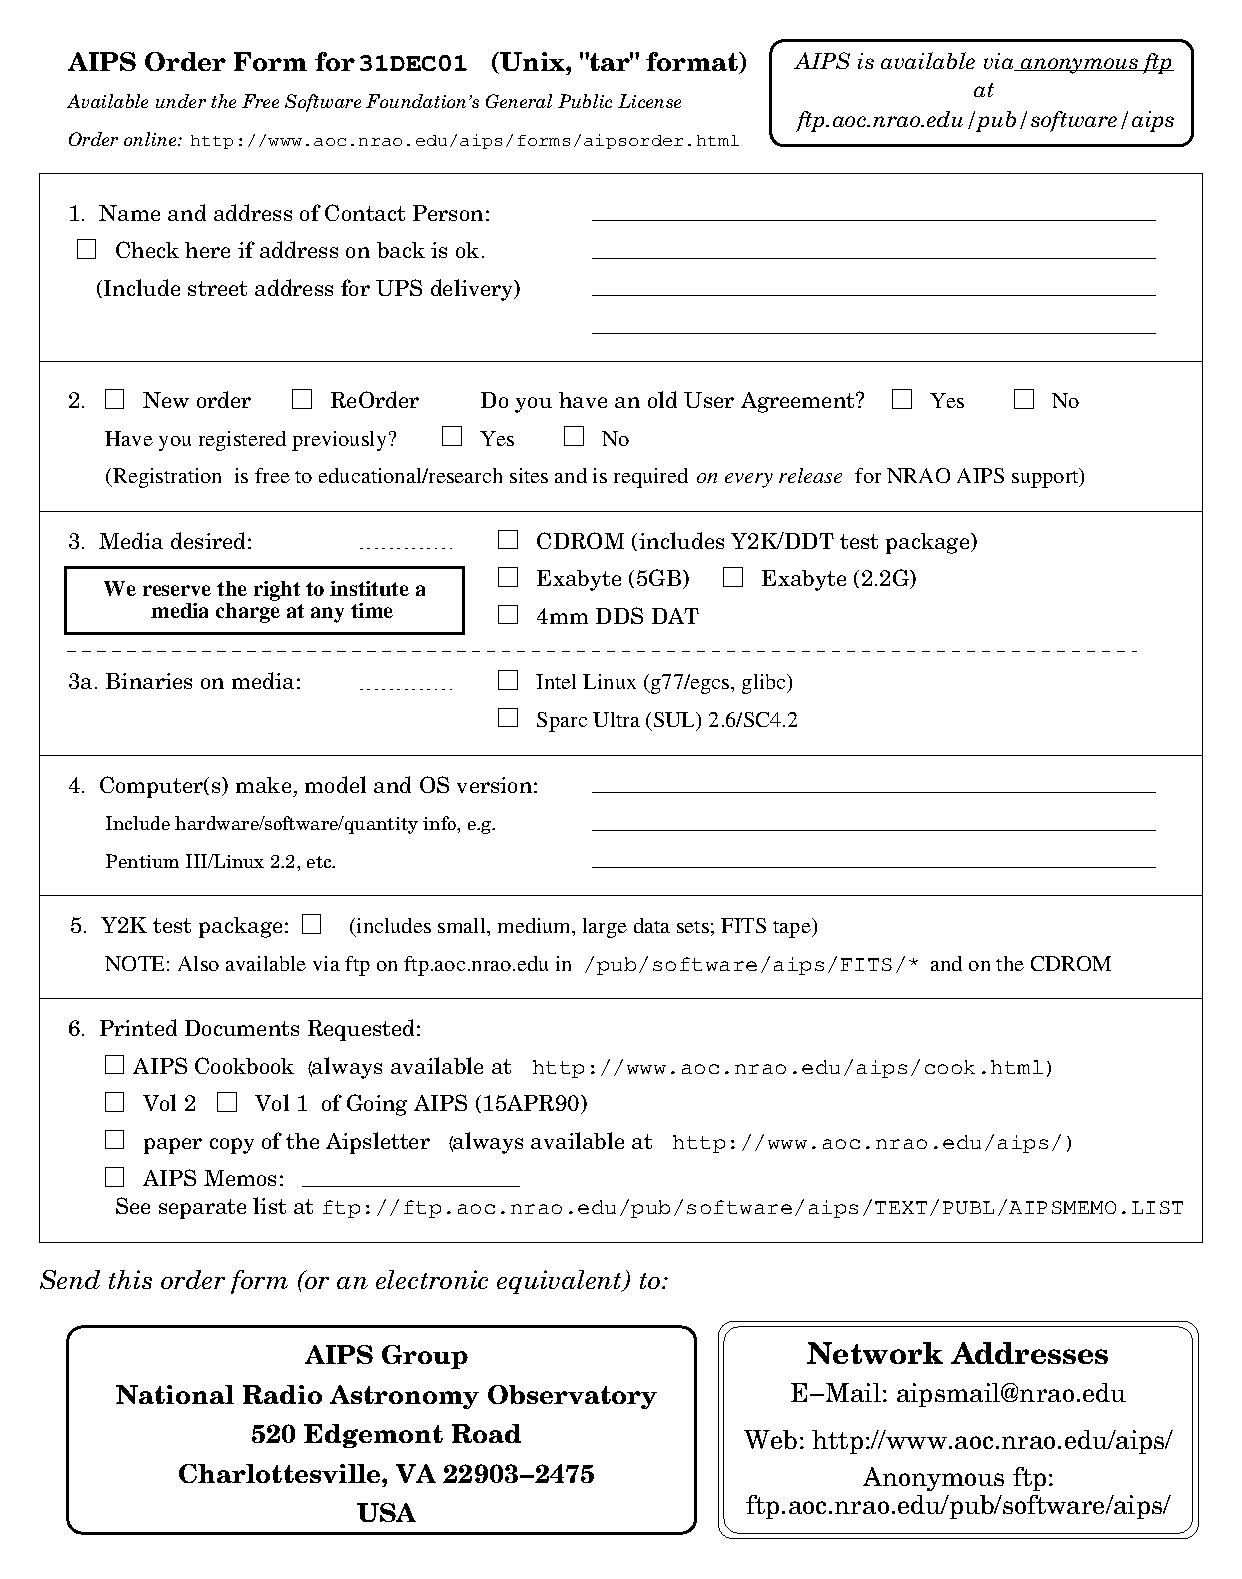
\includegraphics{FIG/AIPSORDER.PS}}}
 \vfill\eject
 \vbox to 4.4in{
  \vfill
  \centerline{\resizebox{!}{2.6in}{\includegraphics{FIG/Mandrill.eps}}}
  \vspace{12pt}
  \centerline{{\huge \tt \AIPRELEASE}}
  \vspace{12pt}
  \vfill}
\phantom{...}
\centerline{\resizebox{!}{!}{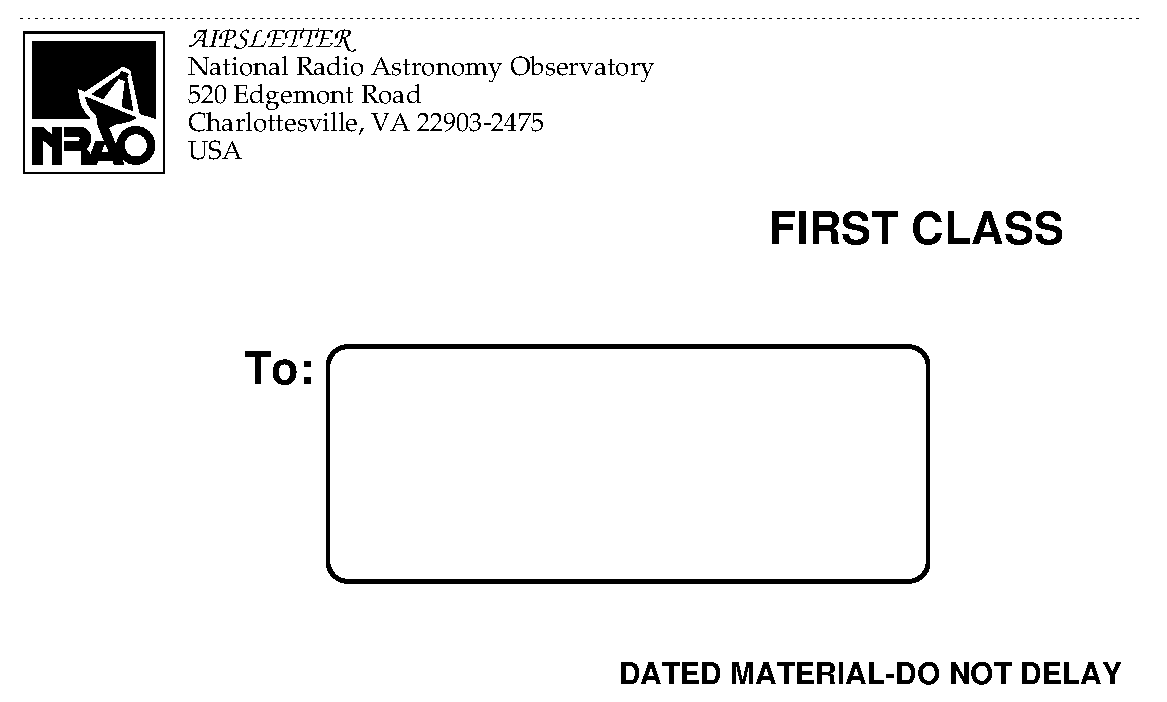
\includegraphics{FIG/AIPSLETM.PS}}}

\end{document}
